% Created by tikzDevice version 0.12.4 on 2023-07-06 13:18:38
% !TEX encoding = UTF-8 Unicode
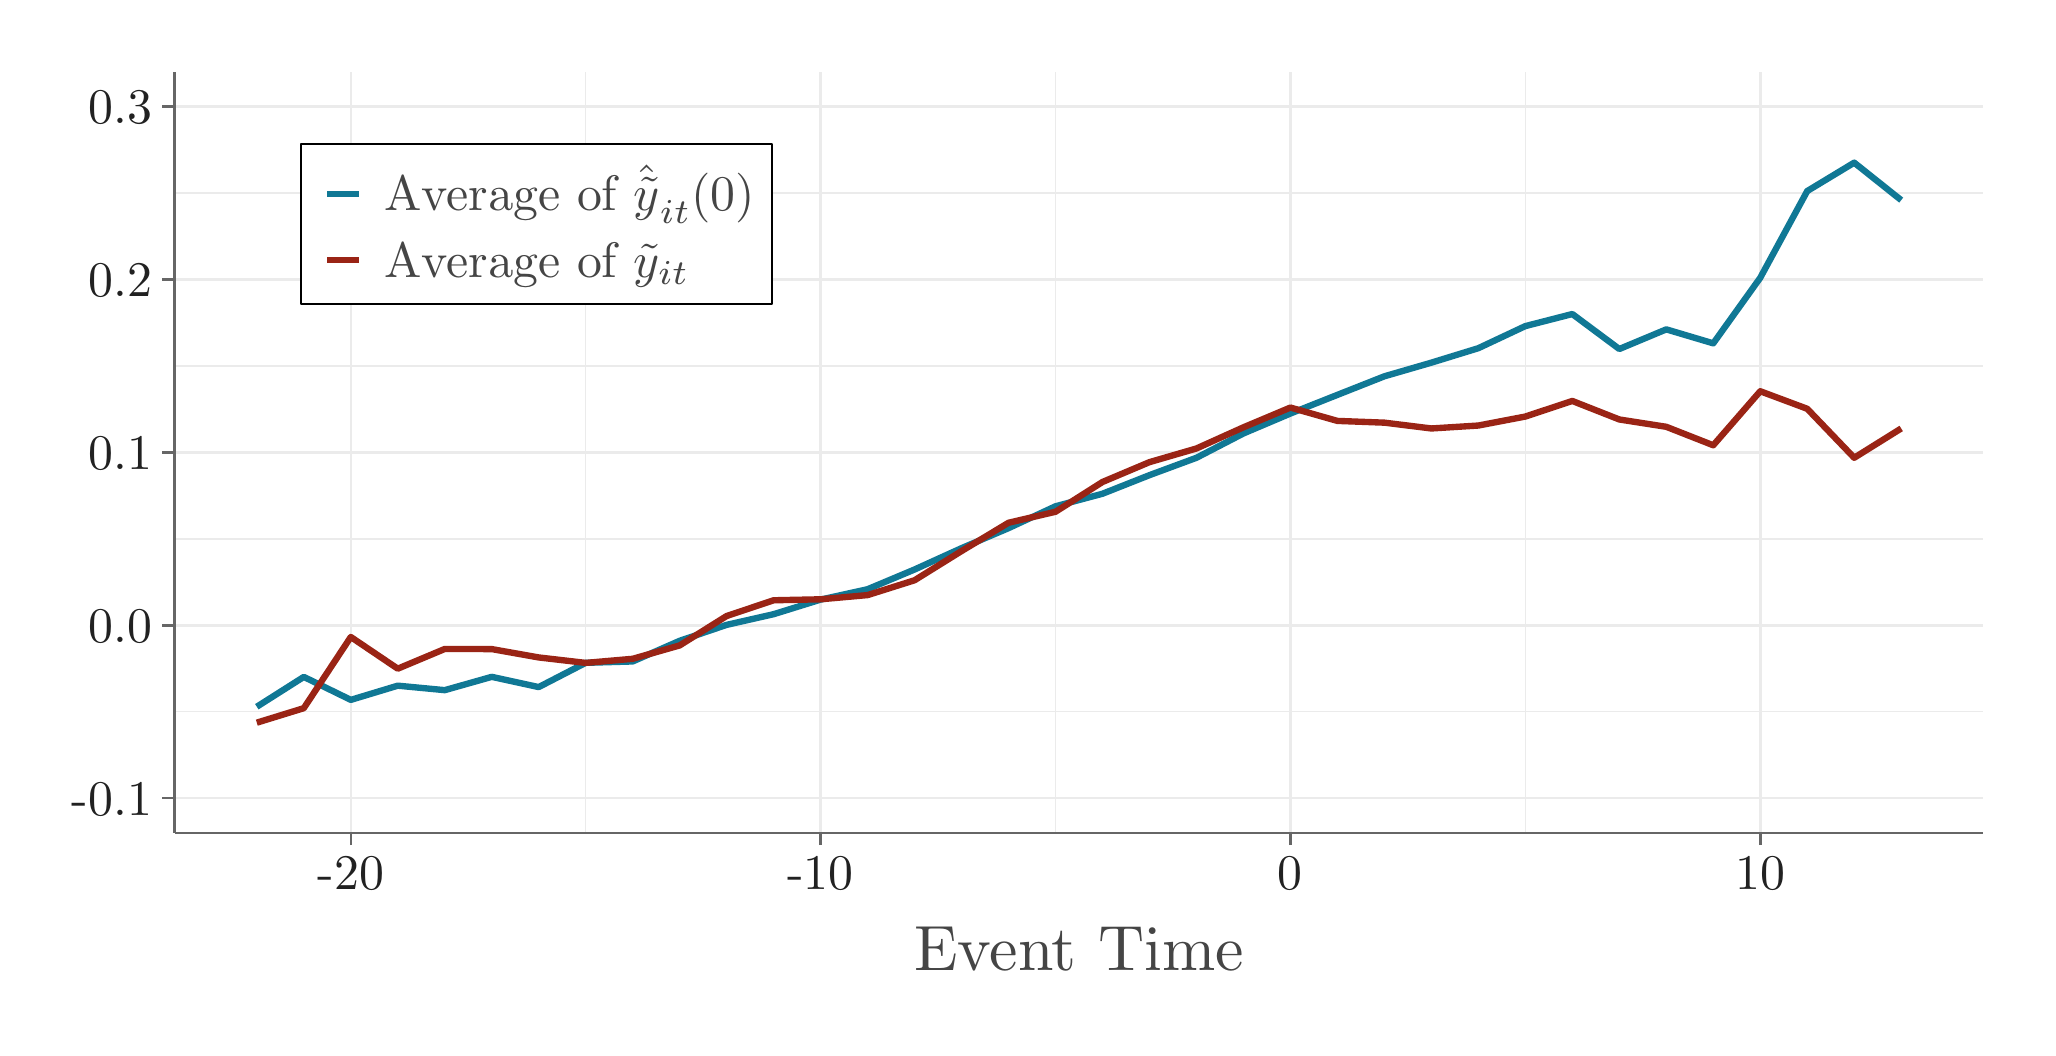
\begin{tikzpicture}[x=1pt,y=1pt]
\definecolor{fillColor}{RGB}{255,255,255}
\path[use as bounding box,fill=fillColor,fill opacity=0.00] (0,0) rectangle (722.70,361.35);
\begin{scope}
\path[clip] (  0.00,  0.00) rectangle (722.70,361.35);
\definecolor{fillColor}{RGB}{255,255,255}

\path[fill=fillColor] (  0.00, -0.00) rectangle (722.70,361.35);
\end{scope}
\begin{scope}
\path[clip] ( 53.09, 70.42) rectangle (706.70,345.35);
\definecolor{fillColor}{RGB}{255,255,255}

\path[fill=fillColor] ( 53.09, 70.42) rectangle (706.70,345.35);
\definecolor{drawColor}{gray}{0.92}

\path[draw=drawColor,line width= 0.5pt,line join=round] ( 53.09,114.16) --
	(706.70,114.16);

\path[draw=drawColor,line width= 0.5pt,line join=round] ( 53.09,176.64) --
	(706.70,176.64);

\path[draw=drawColor,line width= 0.5pt,line join=round] ( 53.09,239.13) --
	(706.70,239.13);

\path[draw=drawColor,line width= 0.5pt,line join=round] ( 53.09,301.61) --
	(706.70,301.61);

\path[draw=drawColor,line width= 0.5pt,line join=round] (201.64, 70.42) --
	(201.64,345.35);

\path[draw=drawColor,line width= 0.5pt,line join=round] (371.41, 70.42) --
	(371.41,345.35);

\path[draw=drawColor,line width= 0.5pt,line join=round] (541.18, 70.42) --
	(541.18,345.35);

\path[draw=drawColor,line width= 0.9pt,line join=round] ( 53.09, 82.92) --
	(706.70, 82.92);

\path[draw=drawColor,line width= 0.9pt,line join=round] ( 53.09,145.40) --
	(706.70,145.40);

\path[draw=drawColor,line width= 0.9pt,line join=round] ( 53.09,207.89) --
	(706.70,207.89);

\path[draw=drawColor,line width= 0.9pt,line join=round] ( 53.09,270.37) --
	(706.70,270.37);

\path[draw=drawColor,line width= 0.9pt,line join=round] ( 53.09,332.85) --
	(706.70,332.85);

\path[draw=drawColor,line width= 0.9pt,line join=round] (116.76, 70.42) --
	(116.76,345.35);

\path[draw=drawColor,line width= 0.9pt,line join=round] (286.52, 70.42) --
	(286.52,345.35);

\path[draw=drawColor,line width= 0.9pt,line join=round] (456.29, 70.42) --
	(456.29,345.35);

\path[draw=drawColor,line width= 0.9pt,line join=round] (626.06, 70.42) --
	(626.06,345.35);
\definecolor{drawColor}{RGB}{16,120,149}

\path[draw=drawColor,line width= 2.3pt,line join=round] ( 82.80,115.97) --
	( 99.78,126.75) --
	(116.76,118.45) --
	(133.73,123.58) --
	(150.71,121.96) --
	(167.69,126.77) --
	(184.66,123.07) --
	(201.64,131.84) --
	(218.62,132.33) --
	(235.59,139.79) --
	(252.57,145.55) --
	(269.55,149.41) --
	(286.52,154.68) --
	(303.50,158.43) --
	(320.48,165.56) --
	(337.45,173.27) --
	(354.43,180.50) --
	(371.41,188.40) --
	(388.38,192.93) --
	(405.36,199.65) --
	(422.34,205.93) --
	(439.32,214.72) --
	(456.29,221.92) --
	(473.27,228.66) --
	(490.25,235.37) --
	(507.22,240.30) --
	(524.20,245.53) --
	(541.18,253.51) --
	(558.15,257.87) --
	(575.13,245.23) --
	(592.11,252.33) --
	(609.08,247.28) --
	(626.06,270.97) --
	(643.04,302.31) --
	(660.01,312.57) --
	(676.99,299.03);
\definecolor{drawColor}{RGB}{154,36,21}

\path[draw=drawColor,line width= 2.3pt,line join=round] ( 82.80,110.21) --
	( 99.78,115.45) --
	(116.76,141.17) --
	(133.73,129.72) --
	(150.71,136.84) --
	(167.69,136.80) --
	(184.66,133.78) --
	(201.64,131.81) --
	(218.62,133.29) --
	(235.59,138.12) --
	(252.57,148.75) --
	(269.55,154.44) --
	(286.52,154.79) --
	(303.50,156.31) --
	(320.48,161.67) --
	(337.45,172.22) --
	(354.43,182.45) --
	(371.41,186.42) --
	(388.38,197.18) --
	(405.36,204.35) --
	(422.34,209.29) --
	(439.32,216.94) --
	(456.29,224.08) --
	(473.27,219.25) --
	(490.25,218.62) --
	(507.22,216.52) --
	(524.20,217.58) --
	(541.18,220.83) --
	(558.15,226.46) --
	(575.13,219.77) --
	(592.11,217.12) --
	(609.08,210.45) --
	(626.06,229.97) --
	(643.04,223.63) --
	(660.01,205.93) --
	(676.99,216.52);

\path[] ( 53.09, 70.42) rectangle (706.70,345.35);
\end{scope}
\begin{scope}
\path[clip] (  0.00,  0.00) rectangle (722.70,361.35);
\definecolor{drawColor}{gray}{0.40}

\path[draw=drawColor,line width= 0.9pt,line join=round] ( 53.09, 70.42) --
	( 53.09,345.35);
\end{scope}
\begin{scope}
\path[clip] (  0.00,  0.00) rectangle (722.70,361.35);
\definecolor{drawColor}{gray}{0.13}

\node[text=drawColor,anchor=base east,inner sep=0pt, outer sep=0pt, scale=  1.80] at ( 44.99, 76.72) {-0.1};

\node[text=drawColor,anchor=base east,inner sep=0pt, outer sep=0pt, scale=  1.80] at ( 44.99,139.20) {0.0};

\node[text=drawColor,anchor=base east,inner sep=0pt, outer sep=0pt, scale=  1.80] at ( 44.99,201.69) {0.1};

\node[text=drawColor,anchor=base east,inner sep=0pt, outer sep=0pt, scale=  1.80] at ( 44.99,264.17) {0.2};

\node[text=drawColor,anchor=base east,inner sep=0pt, outer sep=0pt, scale=  1.80] at ( 44.99,326.65) {0.3};
\end{scope}
\begin{scope}
\path[clip] (  0.00,  0.00) rectangle (722.70,361.35);
\definecolor{drawColor}{gray}{0.40}

\path[draw=drawColor,line width= 0.9pt,line join=round] ( 48.59, 82.92) --
	( 53.09, 82.92);

\path[draw=drawColor,line width= 0.9pt,line join=round] ( 48.59,145.40) --
	( 53.09,145.40);

\path[draw=drawColor,line width= 0.9pt,line join=round] ( 48.59,207.89) --
	( 53.09,207.89);

\path[draw=drawColor,line width= 0.9pt,line join=round] ( 48.59,270.37) --
	( 53.09,270.37);

\path[draw=drawColor,line width= 0.9pt,line join=round] ( 48.59,332.85) --
	( 53.09,332.85);
\end{scope}
\begin{scope}
\path[clip] (  0.00,  0.00) rectangle (722.70,361.35);
\definecolor{drawColor}{gray}{0.40}

\path[draw=drawColor,line width= 0.9pt,line join=round] ( 53.09, 70.42) --
	(706.70, 70.42);
\end{scope}
\begin{scope}
\path[clip] (  0.00,  0.00) rectangle (722.70,361.35);
\definecolor{drawColor}{gray}{0.40}

\path[draw=drawColor,line width= 0.9pt,line join=round] (116.76, 65.92) --
	(116.76, 70.42);

\path[draw=drawColor,line width= 0.9pt,line join=round] (286.52, 65.92) --
	(286.52, 70.42);

\path[draw=drawColor,line width= 0.9pt,line join=round] (456.29, 65.92) --
	(456.29, 70.42);

\path[draw=drawColor,line width= 0.9pt,line join=round] (626.06, 65.92) --
	(626.06, 70.42);
\end{scope}
\begin{scope}
\path[clip] (  0.00,  0.00) rectangle (722.70,361.35);
\definecolor{drawColor}{gray}{0.13}

\node[text=drawColor,anchor=base,inner sep=0pt, outer sep=0pt, scale=  1.80] at (116.76, 49.93) {-20};

\node[text=drawColor,anchor=base,inner sep=0pt, outer sep=0pt, scale=  1.80] at (286.52, 49.93) {-10};

\node[text=drawColor,anchor=base,inner sep=0pt, outer sep=0pt, scale=  1.80] at (456.29, 49.93) {0};

\node[text=drawColor,anchor=base,inner sep=0pt, outer sep=0pt, scale=  1.80] at (626.06, 49.93) {10};
\end{scope}
\begin{scope}
\path[clip] (  0.00,  0.00) rectangle (722.70,361.35);
\definecolor{drawColor}{gray}{0.27}

\node[text=drawColor,anchor=base,inner sep=0pt, outer sep=0pt, scale=  2.31] at (379.90, 20.50) {Event Time};
\end{scope}
\begin{scope}
\path[clip] (  0.00,  0.00) rectangle (722.70,361.35);
\definecolor{drawColor}{RGB}{0,0,0}
\definecolor{fillColor}{RGB}{255,255,255}

\path[draw=drawColor,line width= 0.6pt,line join=round,line cap=round,fill=fillColor] ( 98.75,261.47) rectangle (268.88,319.26);
\end{scope}
\begin{scope}
\path[clip] (  0.00,  0.00) rectangle (722.70,361.35);
\definecolor{fillColor}{RGB}{255,255,255}

\path[fill=fillColor] (106.75,293.36) rectangle (121.21,309.26);
\end{scope}
\begin{scope}
\path[clip] (  0.00,  0.00) rectangle (722.70,361.35);
\definecolor{drawColor}{RGB}{16,120,149}

\path[draw=drawColor,line width= 2.3pt,line join=round] (108.20,301.31) -- (119.76,301.31);
\end{scope}
\begin{scope}
\path[clip] (  0.00,  0.00) rectangle (722.70,361.35);
\definecolor{fillColor}{RGB}{255,255,255}

\path[fill=fillColor] (106.75,269.47) rectangle (121.21,285.36);
\end{scope}
\begin{scope}
\path[clip] (  0.00,  0.00) rectangle (722.70,361.35);
\definecolor{drawColor}{RGB}{154,36,21}

\path[draw=drawColor,line width= 2.3pt,line join=round] (108.20,277.42) -- (119.76,277.42);
\end{scope}
\begin{scope}
\path[clip] (  0.00,  0.00) rectangle (722.70,361.35);
\definecolor{drawColor}{gray}{0.27}

\node[text=drawColor,anchor=base west,inner sep=0pt, outer sep=0pt, scale=  1.80] at (128.95,295.11) {Average of $\hat{\tilde{y}}_{it}(0)$};
\end{scope}
\begin{scope}
\path[clip] (  0.00,  0.00) rectangle (722.70,361.35);
\definecolor{drawColor}{gray}{0.27}

\node[text=drawColor,anchor=base west,inner sep=0pt, outer sep=0pt, scale=  1.80] at (128.95,271.22) {Average of $\tilde{y}_{it}$};
\end{scope}
\end{tikzpicture}
